\graphicspath{{images/}}

\section{\thesection~Discussion}
\label{sec:discussion}

Fitness ranking from competition model fits may be better than from
logistic model fits (Will comparing stripes rankings reveal
anythin?). However, we cannot quantitatively compare fitness estimates
between plates because we are not finding global minima. Work has
begun to develop a genetic algorithm to do so. I am not convinced that
this will succeed because growth is systematically overestimated when
we move from the filled to striped plate for all of the current best
parameter solutions. This suggests an issue with the modelling
approach; below I suggest ways in which this could be improved. In
any case, qualitative cross-plate validation using order of fitness
ranking may still be better (for the competition model).

The first thing to notice about QFA data - from P15, the striped
plate, and the filled plate - is the characteristic endpoint in growth
on each plate. This holds whether a region contains many fast growing
cultures or not. This suggests a plate-level growth-limiting
effect. This could conceivably be an experimental limitation such as
the drying out of an agar plate over time. However, comparison of the
striped and filled data, shows that cultures tend to grow larger when
neighbours are removed and this suggests a direct interaction between
cultures. The strongest candidates are competition for nutrients and
growth limiting signalling such as ethanol poisoning. It is possible
that other growth limiting effects may exist and could confound any
attempt to fit a model which accounts for just one of these. It makes
sense to investigate each likely effect in turn to determine its
contribution and to start by validating the independent limit.



Spots can grow after a long time. Must be nutrients remaining or an
encroachment? I have an image for the stripes plate showing cultures
growing and believe after a very late stage. I need to check the data
images but this may just be encroachment of another culture.
\graphicspath{{images/stripes/}}
\begin{Figure}
  \centering
  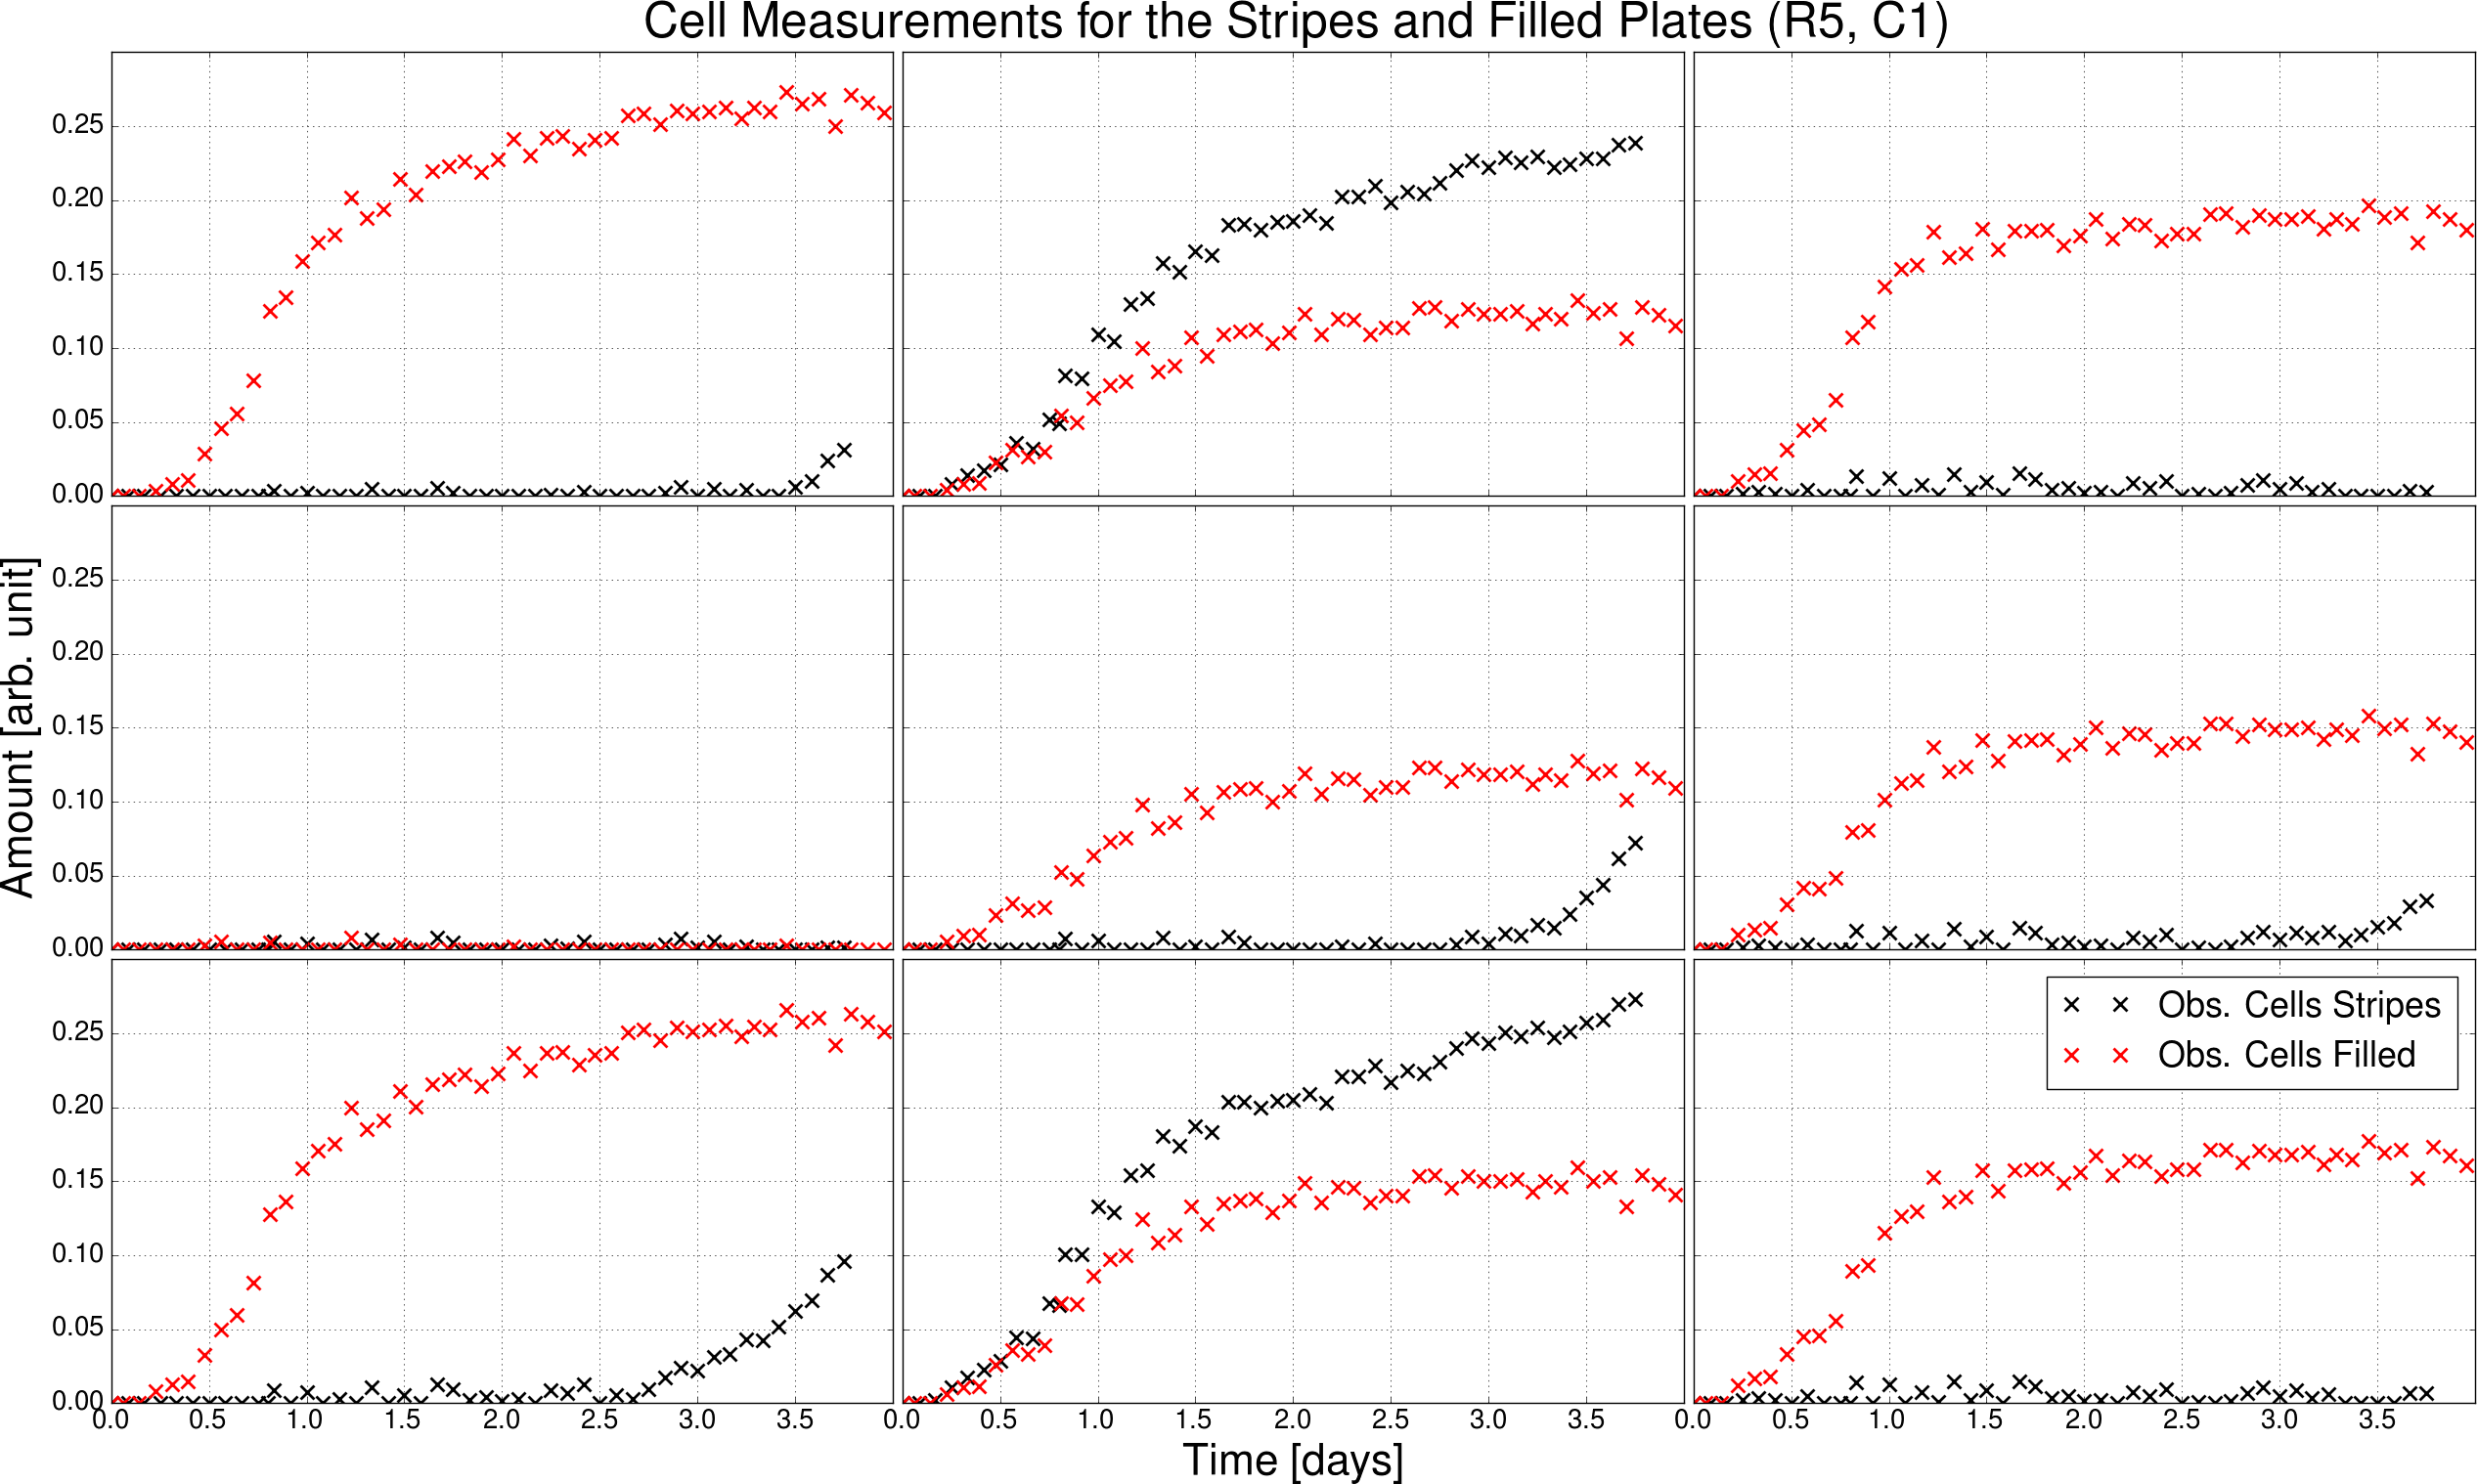
\includegraphics[width=\linewidth]{final/c_meas_r5_c1}
  \captionof{figure}{Observed cells for (R5, C1) 3x3 zone of Stripes
    and Filled plates showing (for Stripes data) slow growing cultures
    starting to grow after faster growing cultures have reached the
    stationary phase.}
  \label{fig:kn_guessing}
\end{Figure}


We have only studied data where cultures are grown in an array on
solid agar where we cannot validate the independent limit. In this
limit, our model says that nutrients can only be converted to cells
and all cultures starting with the same amount of nutrients will reach
the same final cell density. This ignores metabolism which may differ
between strains. Cell arrest could also limit growth. If present,
differences in such effects could account entirely for differences in
final cell density. However, they are unlikely to be the only effect,
because this would not lead to the observed characteristic endpoint in
growth. Using one-culture spot tests (in a perti-dish on ager?) or
liquid cultures we can grow cultures independently and validate the
independent limit. A current issue with methods for estimating
fitness, is that identical strains grow differently on agar or in
liquid culture leading to different fitness rankings (cite). This
problem need not affect our validation as we can simply define a
culture to have different parameters for growth in either medium. A
greater difference may be caused by the dimensionality of the
environment. Mass action kinetics is derived for reactions in a
three-dimentsional (gas or fluid?) (Guldberg and Waage C.M. Guldberg
and P. Waage, Studies Concerning Affinity, C. M. Forhandlinger:
Videnskabs-Selskabet i Christiana (1864), 35) and this approximation
is more valid for liquid cultures than for cultures spotted onto a
surface. I suggest to study first the more ideal case of liquid cultures
and later see if the model holds for cultures grown on a surface. If
it does not, it may be necessary to use a fractal kinetics model or
consider a more detailed model of diffusion of nutrients in agar (if
the reaction is diffusion limited) (I have references for this from
the proposal).

// Model equations for metabolism.//

Reo and Korolev (2014) simulate nutrient dependent growth of a single
bacterial culture on a pertri dish using the diffusion equation and
Neumann and Dirichlet boundary conditions. They create a sink for
nutrients from culture growth and equate the rate of increase in
culture size with the flux of nutrients through the culture area. They
model culture area as varying and keep culture density constant. We
may instead keep culture are area constant, allow culture density to
vary and use our mass action kinetic model to determine the nutrient
sink and culture growth. Simulating or fitting this model could help
us learn about diffusion in QFA experiments. I am interested to know
whether growth becomes diffusion limited at some point before
nutrients are fully depleted. It is probably unfeasible to use such a
detailed model to fit a whole plate because of the computational time
this would take. However, it may be possible to use a finer grid to
increase compartmentalisation of nutrients if this is necessary. This
may extend the validity of the competition model over a larger range
of culture growth rates (for instance when cultures are left empty)
(probably a mistake to leave cultures completely empty in validation
plot; should have instead just used weaker growers to induce a smaller
change).



//Talk about an improvement to the imaginary neighbour model.//




(experiments could be designed to study variation in timescales over
regions of a plate)

% also talk about computational limitations of more complicated
% modelling approaches. Can do this when describing the motivation for
% the fought for model.

\subsection{\thesubsection~Subsection}

%%% Local Variables:
%%% mode: latex
%%% TeX-master: "report"
%%% End:
